\documentclass{beamer}
%pacchetti
\usepackage[T1]{fontenc}
\usepackage[utf8]{inputenc}
\usepackage{graphicx}
\usepackage[italian]{babel}
\usepackage{mathrsfs}
\usepackage{booktabs}
\usepackage{amsmath}
\usepackage{amsfonts}
\usepackage{amssymb}
\usepackage{amsbsy}
\usepackage{amsthm}
\usepackage{enumerate}
\usepackage{quoting}
\quotingsetup{font=small}
\usepackage{diagbox}
\usepackage{graphicx}
\usepackage{setspace}
\usepackage{float}
\usepackage{version}
\usepackage{multicol}
\usepackage{beamerfoils}

\usepackage[none]{hyphenat} %avoid hyphenation
\usepackage{xcolor} %to uset \textcolor
\usepackage{bbm} %funzione indicatrice
% end pacchetti

\usetheme[bgphoto]{polimi}

% Full instructions available at:
% https://github.com/elauksap/beamerthemepolimi

% Set custom font (requires to compile with XeLaTeX).
\usepackage{ifxetex}
\ifxetex
\usepackage{fontspec}
\setsansfont[Scale=0.9]{Arial}
\fi

\usepackage{lipsum}


\newcommand\mynum[1]{%
	\usebeamercolor{enumerate item}%
	\tikzset{beameritem/.style={circle,inner sep=0,minimum size=2ex,text=enumerate item.bg,fill=enumerate item.fg,font=\footnotesize}}%
	\tikz[baseline=(n.base)]\node(n)[beameritem]{#1};%
}


\title{Coupled Markov chains with applications to Approximate Bayesian Computation for model based clustering}
%\subtitle{Subtitle}
\author{E. Bertoni, M. Caldarini, F. Di Filippo, G. Gabrielli, E. Musiari}
\date{11 november 2021}


%Cose da fare

% Mettere biografia
% Mettere \pause e colori
% Sistemare il titolo e layout

\begin{document}

\begin{frame}
\maketitle
\end{frame}

\begin{section}{Introduction}

	\begin{frame}
		\frametitle{A complex problem}

 		\begin{minipage}{0.45\textwidth}
 			\begin{center}
 				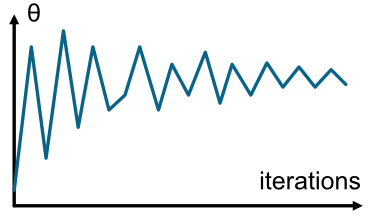
\includegraphics{img/markov_singola}
 			\end{center}
 		\end{minipage}
 		\hfill
 	 	\begin{minipage}{0.45\textwidth}
 	 		\begin{center}
 	 			\only<2>{ 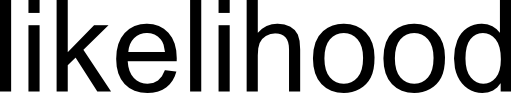
\includegraphics{img/likelihood} }
 	 			\only<3,4,5>{
\includegraphics{img/likelihood_na} }
 	 		\end{center}
 		\end{minipage}
 		
 		\vspace{1cm}
 		
 		\only<4,5>{\begin{minipage}{0.45\textwidth}
 			\begin{center}
 				$\Downarrow$

 				\textbf{Unbiased Markov chain Monte Carlo methods with couplings}
 			\end{center}
 		\end{minipage}}
 		\hfill
 		\only<5>{\begin{minipage}{0.45\textwidth}
 			\begin{center}
 				$\Downarrow$
 				
 				 \textbf{Approximate Bayesian Computation}
 			\end{center}
 		\end{minipage} }
 	 	
 	 	\vspace{0.2cm}
 	 	
 	 	\only<4,5>{\begin{minipage}{0.45\textwidth}
 	 		\begin{center}
 	 			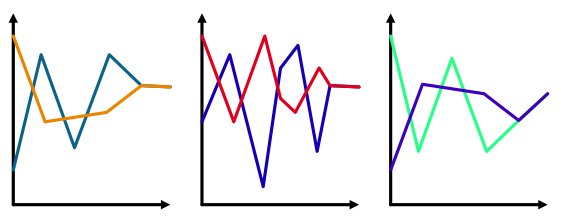
\includegraphics{img/markov_coupled_parallel}
 	 		\end{center}
 	 	\end{minipage}}
 	 	\hfill
 	 	\begin{minipage}{0.45\textwidth}

 	 	\end{minipage}
 	 	
 	 	
 	 	
	\end{frame}

\end{section}

\begin{section}{Unbiased Markov chain Monte Carlo methods with couplings}
	\begin{frame}[plain]{}
		\sectionpage
	\end{frame}

	\begin{frame}
	 	\frametitle{The road to parallelization: coupling of Markov chains}
	 	
	 	$$ \text{Faster MCMC} \implies \text{Parallelization} \pause \iff \text{\textbf{Unbiased estimator}}
	 	$$

		\pause
		\vspace{0.8 cm }
		\begin{minipage}{0.10\textwidth}

		\end{minipage}
		\hfill
		\begin{minipage}{0.45\textwidth}
			Exact estimations algorithms using \textbf{coupling of Markov chain}.
		\end{minipage}
		\hfill
		\begin{minipage}{0.40\textwidth}
			\begin{center}
				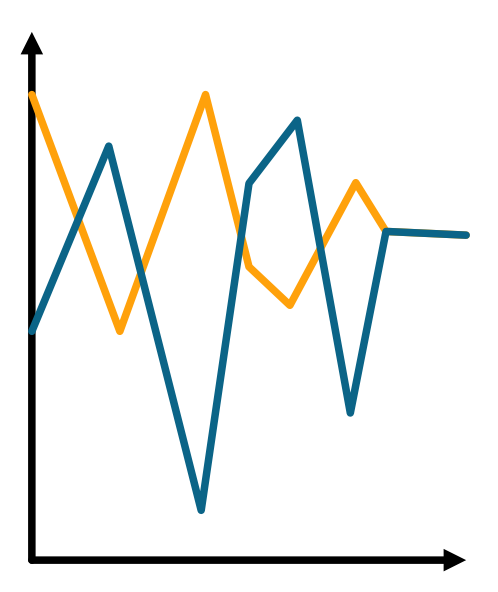
\includegraphics[height=3cm]{img/markov_coupled}
			\end{center}
		\end{minipage}
		
	\end{frame}

	\begin{frame}
	 	\frametitle{Rhee--Glynn estimator I}
	 	The goal is to estimate
	 	$$
	 	\mathbb{E}_{\pi}[h(X)] 
	 	= \int h(x) \pi (\text{d}x)
	 	.
	 	$$
	 	The estimator we are going to construct is based on a coupled pair of Markov chains, $(X_t)_{t\geq 0}$ and $(Y_t)_{t\geq}$, which marginally start from $\pi_0$ and evolve accordingly to $P$.\\ 
	\end{frame}
	
	\begin{frame}{Rhee--Glynn estimator II}
	 	We consider some assumptions:
	 	\begin{enumerate}
	 		\item as $t \to \infty$, 
	 		$$ \mathbb E [h(X_t)] \to \mathbb E_\pi [h(X)];$$
	 		and there exists $\eta > 0$ and $D < \infty$ such that $\mathbb E [|h(X_t)|^{2 + \eta}] \leq D$ for all $t \geq 0$;
	 		
	 		\pause
	 		\item the chains are such that the meeting time 
	 		$$
	 			\tau 
	 			= \inf\{t \geq 1 : X_t = Y_{t-1}\}
	 		$$ 
	 		satisfies $\mathbb{P}(\tau > t) \leq C \delta^t$ for all $t \geq 0$, for some constants $C < \infty$ and $\delta \in (0,1)$;
	 		
	 		\pause
	 		\item the chains stay together after meeting:
	 		$$X_t = Y_{t-1} \text{ for all } t \geq \tau.$$
	 	\end{enumerate}
	\end{frame}
	
	\begin{frame}
	 	\frametitle{Rhee--Glynn estimator III}
	 	Thanks to the previous assumptions we can prove that:
	 	\begin{align*}
	 	\mathbb{E}_{\pi}[h(X)] = \mathbb{E}[
	 		\textcolor{orange}{h(X_k) + \sum_{t = k+1}^{\tau -1}\{h(X_t) - h(Y_{t-1})\} } ]
	 	;
	 	\end{align*}
	 	\pause
	 	and we define the Rhee--Glynn estimator as:
	 	$$ 
	 		H_k(X,Y)
	 		=\textcolor{orange}{ h(X_k) + \sum_{t = k+1}^{\tau -1}\{h(X_t) - h(Y_{t-1})\} }
	 	$$
	 	which is \textbf{unbiased} by construction.
	\end{frame}

	\begin{frame}
	 	\frametitle{Time-averaged estimator I}
		\small {
	 	\only<1>{
		 	$$
		 	H_{k:m}(X,Y)
		 	= \frac{1}{m-k+1}\sum_{l=k}^{m}h(X_l) 
		 	+ \sum_{l=k+1}^{\tau -1}\min(1, \frac{l-k}{m-k+1})\{h(X_l)-h(Y_{l-1})\} 
	 		$$
 		}
	 	\only<2>{
	 		$$
	 		H_{k:m}(X,Y)
	 		= \underbrace{
	 			\frac{1}{m-k+1}\sum_{l=k}^{m}h(X_l) }_{MCMC_{k:m}}
	 		+  
	 			\sum_{l=k+1}^{\tau -1}\min(1, \frac{l-k}{m-k+1})\{h(X_l)-h(Y_{l-1})\} 
	 		$$
 		}
 		\only<3>{
 		$$
 		H_{k:m}(X,Y)
 		= \underbrace{
 			\frac{1}{m-k+1}\sum_{l=k}^{m}h(X_l) }_{MCMC_{k:m}}
 		+ \underbrace{ 
 			\sum_{l=k+1}^{\tau -1}\min(1, \frac{l-k}{m-k+1})\{h(X_l)-h(Y_{l-1})\} }_{BC_{k:m}}
 		$$
 		}
 		}
	 	
	 	\pause
	 	\begin{itemize}
	 		\item $MCMC_{k:m}$  is the standard MCMC average;
	 	\end{itemize}
 	
 		\pause
 		\begin{itemize}
 			\item $BC_{k:m}$ is the bias correction;
 		\end{itemize}
	 	
	\end{frame}

	\begin{frame}
	 	\frametitle{Time-averaged estimator II}

	 	\begin{enumerate}
	 		\item draw $X_0$ and $Y_0$ from an initial distribution $\pi_0$ and draw $X_1 \sim P(X_0, \cdot)$;
	 		\item set $t=1$: while $t<\max\{m,\tau\}$ and:
	 		\begin{itemize}
	 			\item[a] draw $(X_{t+1}, Y_t)\sim \bar P \{(X_t, Y_{t-1}), \cdot \}$; \only<2>{\textcolor{orange}{$\qquad \bar P$ must be evaluated before!}}
	 			\item[b] set $t \leftarrow t+1$;
	 		\end{itemize}
	 		\item compute the time-averaged estimator:
	 		\footnotesize{	 	$$
	 		H_{k:m}(X,Y)
	 		= \frac{1}{m-k+1}\sum_{l=k}^{m}h(X_l) 
	 		+ \sum_{l=k+1}^{\tau -1}\min(1, \frac{l-k}{m-k+1})\{h(X_l)-h(Y_{l-1})\} .
	 		$$
	 		}

	 	\end{enumerate}
	\end{frame}

	\begin{frame} 	
		\frametitle{Time-averaged estimator III}
	 	Metropolis--Hasting algorithm allow us to calculate the coupled kernel $\bar P \{(X_t, Y_{t-1}), \cdot \}$:
	 	\only<1>{
	 	\begin{enumerate}
	 		\item sample $(X^\star, Y^\star) | (X_t, Y_{t-1})$ from a maximal coupling of $q(X_t, \cdot)$ and $q(Y_{t-1}, \cdot)$;
	 		\item sample $U \sim \mathcal{U}([0,1])$;
	 		\item if
	 		$$ U
	 		\leq \min\bigg \{
	 		1,
	 		\frac{ \pi(X^\star)q(X^\star,X_t)}{
	 			\pi(X_t)q(X_t, X^\star)}
	 		\bigg \}
	 		$$
	 		then $X_{t+1} = X^\star$; otherwise $X_t = X_{t-1}$;
	 		\item if
	 		$$ U
	 		\leq \min\bigg \{ 
	 		1,
	 		\frac{ \pi(Y^\star)q(Y^\star,Y_t)}{
	 			\pi(Y_t)q(Y_t, Y^\star)}
	 		\bigg \}
	 		$$
	 		then $Y_{t+1} = Y^\star$; otherwise $Y_t = Y_{t-1}$.
	 	
	 	\end{enumerate}
 		}
 		\only<2>{
 			\begin{enumerate}
 				\item sample $(X^\star, Y^\star) | (X_t, Y_{t-1})$ from a maximal coupling of $q(X_t, \cdot)$ and $q(Y_{t-1}, \cdot)$;
 				\item sample $\textcolor{orange}{U} \sim \mathcal{U}([0,1])$;
 				\item if
 				$$ \textcolor{orange}{U}
 				\leq \min\bigg \{
 				1,
 				\frac{ \pi(X^\star)q(X^\star,X_t)}{
 					\pi(X_t)q(X_t, X^\star)}
 				\bigg \}
 				$$
 				then $X_{t+1} = X^\star$; otherwise $X_t = X_{t-1}$;
 				\item if
 				$$ \textcolor{orange}{U}
 				\leq \min\bigg \{ 
 				1,
 				\frac{ \pi(Y^\star)q(Y^\star,Y_t)}{
 					\pi(Y_t)q(Y_t, Y^\star)}
 				\bigg \}
 				$$
 				then $Y_{t+1} = Y^\star$; otherwise $Y_t = Y_{t-1}$.
 				
 			\end{enumerate}
 		}
	\end{frame}

\end{section}



\begin{section}{Approximate Bayesian Computation}

    \begin{frame}[plain]{}
		\sectionpage
	\end{frame}

	\begin{frame}{Likelihood-free rejection sampling algorithm I}
		\emph{Inputs:}
		\begin{itemize}
			\item a target posterior density $\pi(\theta | y_{obs}) \propto p(y_{obs}|\theta) \pi(\theta)$, consisting of a prior distribution $\pi(\theta)$ and a procedure of generating data under the model $p(y_{obs}|\theta)$;
			\item a proposal density $g(\theta)$, with $g(\theta)\textgreater 0 $ if $\pi(\theta | y_{obs}) \textgreater 0$;
			\item an integer $N > 0$.
		\end{itemize}
		
		\pause
		\emph{Sampling} for $i= 1,..., N$:
			\begin{enumerate}
			\item generate $\theta ^ {(i)} \sim g(\theta)$ from sampling density $g$;
			\item generate $ y \sim p(y|\theta ^ {(i)})$ from the likelihood;
			\item if $y=y_{obs}$, then accept $\theta ^ {(i)}$ with probability $\frac{\pi(\theta ^ {(i)})}{K g(\theta ^ {(i)})}$, where $K \geq \max_{\theta}{\frac{\pi(\theta)}{g(\theta)}}$; else go to \mynum{1}.
		\end{enumerate}
		
		\pause
		\emph{Output:}
		\begin{itemize}
			\item a set of parameter vectors $\theta ^ {(1)},..., \theta ^ {(N)}$ which are samples from $\pi(\theta |y_{obs})$.
		\end{itemize}

	\end{frame}

	\begin{frame}{Likelihood-free rejection sampling algorithm II}
		Is this an efficient method for complex analysis?
		
		\pause
		\vspace{0.3cm}
		\mynum{3} If $\parallel y-y_{obs}\parallel \leq h$, then accept $\theta ^ {(i)}$ with probability $\frac{\pi(\theta ^ {(i)})}{K g(\theta ^ {(i)})}$, where $K \geq \max_{\theta}{\frac{\pi(\theta)}{g(\theta)}}$; 
		else go to \mynum{1}. 
	\end{frame}

	\begin{frame}{Approximate Bayesian Computation}

		\only<1>{$$\pi(\theta, y| y_{obs}) \propto \textcolor{orange}{\mathbbm{1}(\parallel y-y_{obs} \parallel \leq h)}p(y|\theta)\pi(\theta)$$
		\[ \Downarrow \]
		\[		\pi_{ABC}(\theta, y | y_{obs}) \propto \textcolor{orange}{K_h(u)}p(y|\theta)\pi(\theta)\]}
	
		\only<2>{$$\pi(\theta, y| y_{obs}) \propto \mathbb{I}(\parallel y-y_{obs} \parallel \leq h)p(y|\theta)\pi(\theta)$$
		\[ \Downarrow \]
		\[		\pi_{ABC}(\theta, y | y_{obs}) \propto \textcolor{orange}{K_h(u)}p(y|\theta)\pi(\theta)\]}

		\pause
		\vspace{0.7cm}
		Where we used a \textbf{standard smoothing kernel function}:
		\[ \textcolor{orange}{K_h(u)}  =  \frac{1}{h}  K \left( \frac{u}{h} \right), \quad \text{ with } \  u=\parallel y-y_{obs} \parallel \]
		
		
	\end{frame}

	\begin{frame}{Summary statistics I}
		Is this feasible in practice?
		
		\pause
		\vspace{0.3cm}
		No, it's difficult to have $y\approx y_{obs}$: we should use a large $h$, obtaining a poor posterior approximation!
		
		\vspace{0.3cm}
		$\Longrightarrow$ use summary statistics $s = S(y)$
	\end{frame}
		
	\begin{frame}{Summary statistics II}
		
		Critical decision: choice of summary statistics\\
		\pause
		
		\vspace{0.3cm}
		Dimension of summary statistics:
		\begin{itemize}
			\item large enough to contain as much as information about observed data as possible
			\item low enough to avoid curse of dimensionality of matching $s$ and $s_{obs}$
		\end{itemize}
		
		\vspace{0.3cm}
		$\Longrightarrow$ choose sufficient statistics, such that:
		\[   \pi(\theta|s_{obs}) \equiv \pi(\theta|y_{obs})   \]

	\end{frame}

	\begin{frame}{Distance measure}
		Distance measure: substantial impact on ABC algorithm efficiency
		
		\[  \parallel s - s_{obs} \parallel = (s - s_{obs})^\top \Sigma^{-1} (s - s_{obs}) \]
		
		\pause
		\vspace{1cm}
		\begin{itemize}
			\item $\Sigma = $ identity matrix $ \rightarrow$ Euclidean distance 
			\item $\Sigma =$ diagonal matrix of non-zero weights $ \rightarrow$ Weighted Euclidean distance 
			\item $\Sigma = $ full covariance matrix of $s \rightarrow$ Mahalanobis distance 
		\end{itemize}
	\end{frame}

	\begin{frame}{ABC rejection sampling algorithm}

		\only<1> {
			\emph{Inputs:}
			\begin{itemize}
				\item a target posterior density $\pi(\theta | y_{obs}) \propto p(y_{obs}|\theta) \pi(\theta)$, consisting of a prior distribution $\pi(\theta)$ and a procedure of generating data under the model $p(y_{obs}|\theta)$;
				\item a proposal density $g(\theta)$, with $g(\theta)\textgreater 0 $ if $\pi(\theta | y_{obs}) \textgreater 0$;
				\item an integer $N \textgreater0$;
				\item a kernel function $K_h(u)$ and a scale parameter $h > 0$;
				\item a low dimensional vector of summary statistics $s=S(y)$.
			\end{itemize}
		}
		\only<2> {
			\emph{Sampling} for $i= 1,..., N$:
			\begin{enumerate}
				\item generate $\theta ^ {(i)} \sim g(\theta)$ from sampling density $g$;
				\item generate $ y \sim p(y|\theta ^ {(i)})$ from the likelihood;
				\item compute summary statistic $s = S(y)$;
				\item accept $\theta ^ {(i)}$ with probability $\frac{K_h(\parallel s-s_{obs}\parallel)   \pi(\theta ^ {(i)})}{K g(\theta ^ {(i)})}$, where $K \geq K_h(0)\max_{\theta}{\frac{\pi(\theta)}{g(\theta)}}$; else go to 1.
			\end{enumerate}
		
			\emph{Output:}
			\begin{itemize}
				\item a set of parameter vectors $\theta ^ {(1)},..., \theta ^ {(N)} \sim \pi_{ABC}(\theta |S_{obs})$.
			\end{itemize}
		}
		

	\end{frame}
\end{section}

\begin{section}{Conclusions}
	
    \begin{frame}[plain]{}
		\sectionpage
	\end{frame}

	\begin{frame}{Next steps}
		Our focus till now was to understand the fundamental concepts and collect the missing information.
		
		\vspace{0.5 cm}
		The next step will be a \textbf{simple and separate implementation} of both solution to be tested on simulated data.
		
		\vspace{0.5 cm}
		Further steps will consider the \textbf{integration} of both solution into a single implementation and the testing on more complex data.
	\end{frame}

	\begin{frame}{Bibliography}
		\nocite{*}
		\bibliographystyle{unsrt}
		\tiny{ \bibliography{refs_MCMC,refs_ABC} }

	
%				\begin{minipage}[t]{0.4\textwidth}
%			\footnotesize {Unbiased Markov chain Monte Carlo methods with couplings:}
%			\tiny { \bibliography{refs_MCMC} }
%		\end{minipage}
%		\hfill
%		\begin{minipage}[t]{0.4\textwidth}
%			\footnotesize {Approximate Bayesian computation:}
%			\tiny { \bibliography{refs_ABC} }
%		\end{minipage}

	\end{frame}
\end{section}

\end{document}
